\chapter{Planificación}

A la hora de realizar un proyecto de esta magnitud, la planificación es de suma importancia, ya que a fin de cuentas es el pilar en el que se vertebra el proyecto, y que dicta qué se debe ir haciendo en cada momento. La planificación aquí expuesta ha permitido cumplir los objetivos inicialmente establecidos.
\begin{itemize}
	\item Abril: Definición del proyecto
	\begin{itemize}
		\item Identificación del tema a desarrollar
		\item Formulación de los objetivos
	\end{itemize}
	\item Mayo: Investigación
	\begin{itemize}
		\item Recopilación y revisión de libros y papers relevantes
		\item Búsqueda de información sobre las dos tecnologías de paralelización
	\end{itemize}
	\item Junio: Implementación de OpenMP
	\begin{itemize}
		\item Secuencial
		\item Paralelismo por operaciones
		\item Paralelismo por componentes
		\item Pruebas y validación del código
	\end{itemize}
	\item Julio: Implementación de CUDA
	\begin{itemize}
		\item Desarrollo de los kernels
		\item Kernels Graph
		\item Shuffles y grids
		\item Pruebas y validación del código
	\end{itemize}
	\item Agosto: Memoria del proyecto
	\begin{itemize}
		\item Mediciones temporales
		\item Análisis de los datos
		\item Redacción de la memoria
	\end{itemize}
	\item Septiembre: Entrega
	\begin{itemize}
		\item Últimas correcciones
		\item Presentación y defensa
	\end{itemize}
\end{itemize}

\begin{figure}[H]
	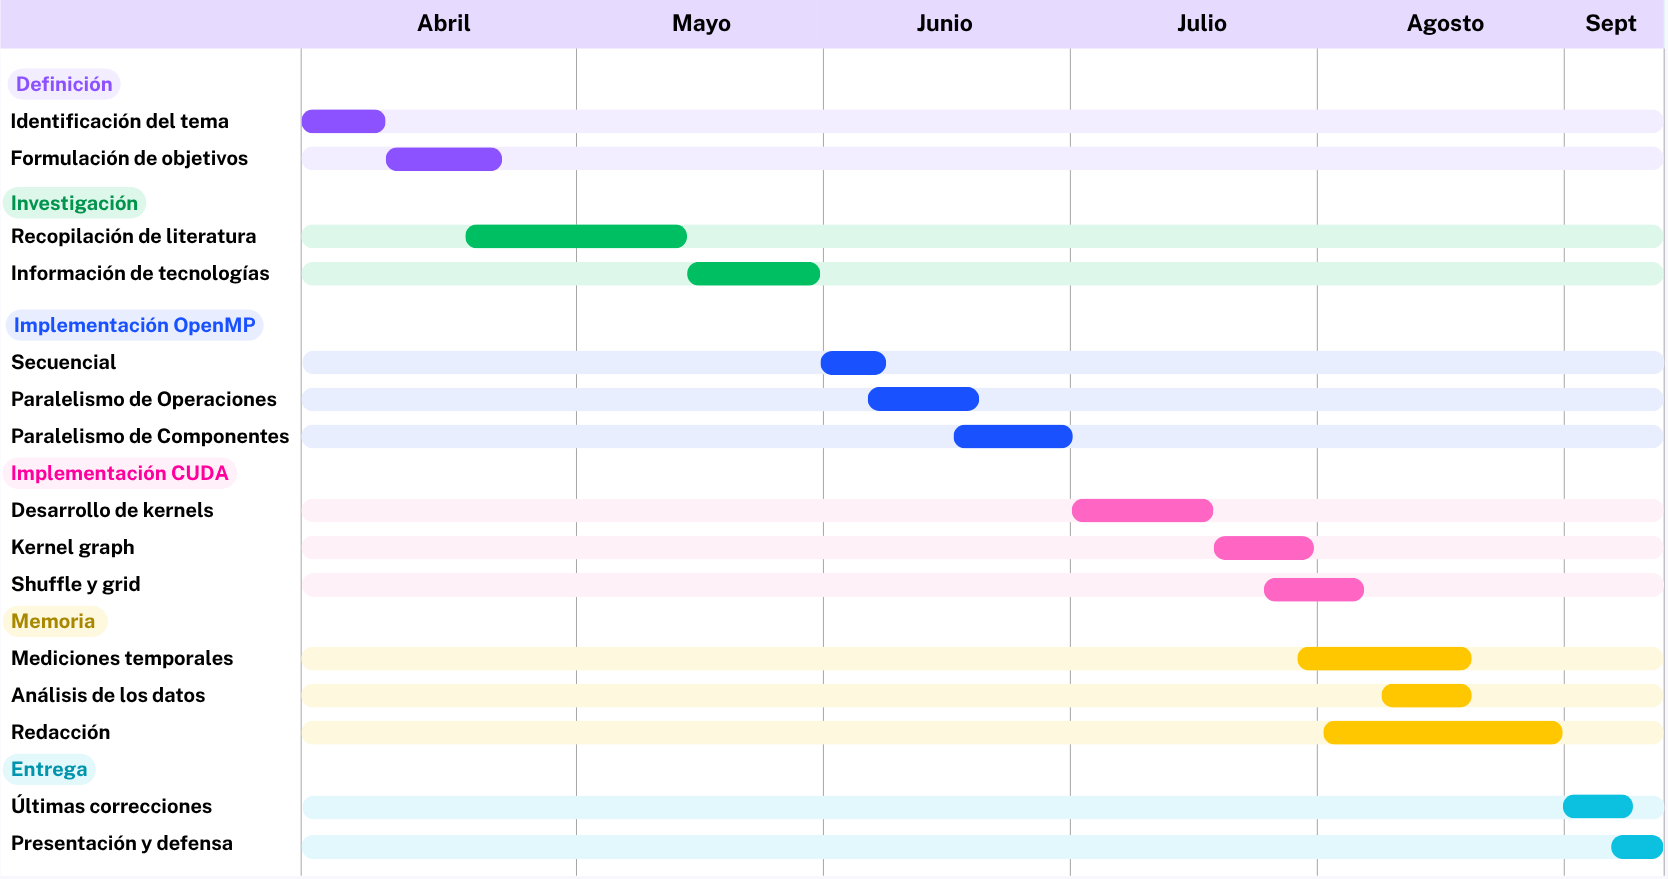
\includegraphics[width=\linewidth]{imagenes/Diagrama-Gantt.png}
	\caption{Diagrama de Gantt}
	\label{fig:Diagrama-Gantt}
\end{figure}

\chapter{Código fuente}

El código desarrollado, así como las diferentes partes que componen esta memoria se encuentran el el siguiente repositorio:

\url{https://github.com/PepeNavarro7/TFG}

GitHub es una plataforma online donde los desarrolladores almacenan, comparten y colaboran en proyectos de programación usando Git, que es un sistema de control de versiones distribuido, que sirve para guardar el historial de un proyecto, comparar versiones, volver atrás, trabajar en paralelo y fusionar cambios sin perder nada.

Para usar el proyecto, basta con descargar cualquiera de las dos carpetas del solver (OpenMP o CUDA), y ejecutar el Makefile siguiendo las intrucciones que vienen dentro del mismo, que permiten la ejecución de un solo test, o de una batería de ellos.

Para las mediciones que se muestran en el presente proyecto se utilizó ese mismo código fuente ejecutado desde el sistema \textit{ILEX} perteneciente a la Universidad de Granada.